\documentclass{article}

% RAAAI 2026 requires the NeurIPS 2026 format and double-blind review.
% Keep "final" and "preprint" disabled for the review submission.
% Use numeric citations, ordered and compressed by natbib.
\PassOptionsToPackage{numbers,sort&compress}{natbib}
\usepackage[dblblindworkshop]{neurips_2026}
\workshoptitle{Workshop on Resource-Aware Agentic AI (RAAAI) at NeurIPS 2026}

% Encoding settings from the official NeurIPS 2026 template.
\usepackage[utf8]{inputenc}
\usepackage[T1]{fontenc}

% Personal packages and presentation macros.
\usepackage{xcolor}

\definecolor{linkpurple}{RGB}{90,40,90}
\definecolor{pdrblue}{RGB}{37,99,235}
\definecolor{green}{HTML}{10B981}

\usepackage{hyperref}       % hyperlinks
\hypersetup{
  colorlinks=true,
  linkcolor=linkpurple,
  citecolor=green!50!black,
  urlcolor=blue!50!black
}
 
\usepackage{url}            % simple URL typesetting
\usepackage{booktabs}       % professional-quality tables
\usepackage{amsfonts}       % blackboard math symbols
\usepackage{nicefrac}       % compact symbols for 1/2, etc.
\usepackage{microtype}      % microtypography
% \usepackage[svgnames]{xcolor}         % colors

\usepackage{amsmath,amssymb}
\usepackage{mathtools}
\usepackage{amsthm}
\usepackage{bm}
\usepackage{enumitem}
\usepackage{ulem}
\usepackage{cleveref}
\usepackage{pifont}
\usepackage[most]{tcolorbox}

\usepackage{algorithm}
\usepackage{algpseudocode}

% package for table
\usepackage{multirow}
\usepackage{caption} 
% \captionsetup[table]{skip=10pt}
\usepackage{adjustbox}
\usepackage{color, colortbl}
\usepackage{subcaption}
\usepackage{graphicx}
\usepackage{makecell}

% package for wraptable
\usepackage{wrapfig,lipsum}

% package for theorem
\newtheorem{theorem}{Theorem}
\newtheorem{lemma}{Lemma}
\newtheorem{assumption}{Assumption}
\newtheorem{corollary}{Corollary}
\newtheorem{definition}{Definition}
\newtheorem{proposition}{Proposition}
\newtheorem{remark}{Remark}

%% takeaway box
\newtcolorbox{takeaway}{
  enhanced,
  colback=pdrblue!4,
  colframe=pdrblue!70!black,
  boxrule=0.75pt,
  arc=1.8pt,
  left=6pt,right=6pt,top=4pt,bottom=4pt,
  before skip=6pt,after skip=7pt,
  fontupper=\small
}

% Draft-review markers. Keep draft mode on while writing. In clean mode,
% revisions become plain text and every unresolved marker stops the build.
\newif\ifdraftmarks
\draftmarksfalse
\definecolor{draftrevision}{HTML}{2563EB}
\definecolor{draftpending}{HTML}{7C3AED}
\definecolor{draftplaceholder}{HTML}{DC2626}
\definecolor{draftverify}{HTML}{D97706}

\newcommand{\draftmarkererror}[1]{%
  \PackageError{RAAAI draft markers}{Unresolved #1 marker remains}{%
    Resolve this marker before building the clean submission copy.}%
}
\newcommand{\cd}[1]{%
  \ifdraftmarks\textcolor{draftrevision}{#1}\else#1\fi%
}
\newcommand{\rev}[1]{\cd{#1}}
\newcommand{\resultpending}[1]{%
  \ifdraftmarks
    \textcolor{draftpending}{[\textbf{RESULT PENDING}: #1]}%
  \else
    \draftmarkererror{RESULT PENDING}%
  \fi%
}
\newcommand{\placeholder}[1]{%
  \ifdraftmarks
    \textcolor{draftplaceholder}{[\textbf{PLACEHOLDER}: #1]}%
  \else
    \draftmarkererror{PLACEHOLDER}%
  \fi%
}
\newcommand{\verify}[1]{%
  \ifdraftmarks
    \textcolor{draftverify}{[\textbf{VERIFY}: #1]}%
  \else
    \draftmarkererror{VERIFY}%
  \fi%
}
\newcommand{\pendingcell}[1]{%
  \ifdraftmarks
    \cellcolor{draftpending!12}%
    \textcolor{draftpending}{\textbf{\scriptsize pending}}%
  \else
    \draftmarkererror{RESULT PENDING (#1)}%
  \fi%
}

\definecolor{avgrowgray}{gray}{0.9}
\newcolumntype{a}{>{\columncolor{avgrowgray}}c}

\definecolor{gaegreen}{HTML}{10B981}
\definecolor{gaerowhighlight}{HTML}{E6F9F1}

% \newtheorem{definition}{Definition}
% \newtheorem{proposition}{Proposition}
% \newtheorem{remark}{Remark}

\newcommand{\new}[1]{\textbf{\textcolor{blue}{#1}}}
\newcommand{\hl}[1]{\textbf{\textcolor{teal}{#1}}}
\newcommand{\open}[1]{\textbf{\textcolor{orange}{[Open] #1}}}
\newcommand{\todo}[1]{\textbf{\textcolor{red}{[TODO] #1}}}
\newcommand{\hypo}[1]{\textbf{\textcolor{violet}{[Hypothesis] #1}}}


% Show review and unresolved-work markers in working PDFs. Before submission,
% switch to \draftmarksfalse; unresolved markers will then stop the build.
\draftmarkstrue

% Add a separate notation file here when it is available.
% \input{macros}

\title{Finite-$K$ Posterior Learning with One-Draw Primal Updates}

% The dblblindworkshop option anonymizes the review copy.
\author{Anonymous Author(s)}

\begin{document}

\maketitle

\begin{abstract}
Multi-sample reasoning improves reliability by generating several candidate solutions, increasing the chance that at least one succeeds within a limited inference budget.
The candidate pool's success depends on which solver variants it contains, so we model their distribution as a regularized posterior over solver parameters.
Each posterior draw instantiates one candidate solver, and we optimize the posterior to increase the chance that at least one candidate succeeds.
Direct optimization of this objective requires several sampled solvers in every update, so we use a Fenchel reformulation and a Bregman update to learn from one posterior draw and a running summary of each problem's failures.
This keeps the number of solver executions per training update independent of the size of the candidate pool.
Across challenging reasoning tasks, our method improves candidate coverage and, in a controlled comparison, achieves performance comparable to multi-draw training with lower training cost.
\end{abstract}


\section{Introduction}
\label{sec:introduction}

Complex reasoning problems often admit several solution paths, and a single
solver execution can fail even when another would succeed. Multi-sample
inference reduces this risk by generating several candidate solutions and
selecting or aggregating them, as in repeated sampling, self-consistency, and
verifier-guided
reasoning~\citep{chen2021codex,wang2023selfconsistency,cobbe2021verifiers}.
With a limited inference budget, the candidate pool succeeds when at least one
candidate solves the problem. Repeated sampling can substantially expand
problem coverage, although its gains depend on how candidates are generated
and selected~\citep{brown2024monkeys,snell2024scaling,wu2025inferencescaling}.
Recent training methods therefore score groups of outputs jointly or tailor
fine-tuning to multi-sample
selection~\citep{pmlr-v267-tang25o,walder2025pkpo,chow2025inferenceaware,chen2025rethinking}.
This line of work treats candidate-pool success as a training target rather
than only an inference-time metric.

A posterior over solver parameters naturally supplies the multiple candidates
used at inference. Each posterior draw instantiates a complete solver that
produces one candidate solution, so repeated draws assemble the inference pool
from a single learned distribution. We learn this distribution as a
regularized posterior, combining task loss with regularization toward a
prior~\citep{bissiri2016general,blundell2015weight,shen2024variational}.
The posterior's probability mass determines which solver variants appear in
the pool and how often they are sampled, so optimizing it directly shapes the
candidate generator used at inference.
Variational posterior learning typically optimizes the expected loss of one
sampled model. For multi-sample inference, we instead introduce finite-$K$
posterior learning, which trains the regularized posterior to make a finite
candidate pool more likely to contain at least one successful solution. Direct
optimization of this pool-level objective requires several posterior-sampled
solvers in every update, so its cost grows with the target pool size.

We reduce this cost with a Fenchel reformulation and a Bregman update that
require only one posterior draw per training update. The Fenchel reformulation
expresses the pool-level objective so that one sampled solver can update the
posterior when its failure is weighted by how likely the other candidates are
to fail. The required weight differs across problems and changes as the
posterior learns because sampled solvers do not fail equally often on every
problem. Estimating it from several fresh draws would cancel the computational
saving. We therefore maintain, for each training problem, a running summary of
how often its sampled solvers fail. A closed-form Bregman update refreshes this
summary after each observed failure, so the current summary guides the
posterior update and the new observation informs the next visit. The procedure
needs neither an inner optimization loop nor another solver execution. Each
update uses one sampled solver regardless of the candidate-pool size.

Across challenging reasoning tasks, our method improves candidate coverage
and, in a controlled comparison, achieves performance comparable to direct
multi-draw training with lower training cost. Our contributions are:

\begin{itemize}
  \item We formulate finite-$K$ posterior learning for reasoning, aligning a
  regularized posterior over solver parameters with the collective success of
  the finite candidate pool used at inference.

  \item We derive an exact Fenchel reformulation of the differentiable
  finite-$K$ objective that enables posterior updates from one sampled solver,
  guided by a problem-specific summary of posterior failures.

  \item We derive a closed-form Bregman update for tracking these failure
  summaries and analyze how sampling noise and posterior drift affect their
  tracking error and the resulting finite-$K$ objective gap.
\end{itemize}

\section{Related work}
\label{sec:related-work}
% Cover multi-sample inference, generalized/loss-calibrated Bayes,
% variational learning, and stochastic primal--dual optimization.

\subsection{Multi-sample Inference and Test-time Scaling}
\label{sec:related-multisample}

Multi-sample inference improves performance by generating multiple candidate solutions and aggregating their complementary outcomes.
Its benefit was quantified in code generation through Pass@$K$, which measures whether at least one sampled program passes the tests~\citep{chen2021codex}.
For reasoning tasks, self-consistency aggregates diverse reasoning paths through answer-level voting~\citep{wang2023selfconsistency}, while outcome and process verifiers rank candidate solutions using learned correctness signals~\citep{cobbe2021verifiers,lightman2024verify}.
Structured search methods further extend this principle by expanding and pruning intermediate reasoning branches instead of sampling complete solutions independently~\citep{yao2023tree}.
These inference procedures can be viewed as forms of test-time scaling that allocate additional compute to broader candidate exploration.
Repeated-sampling studies demonstrate that increasing the number of attempts can substantially expand problem coverage~\citep{brown2024monkeys}, whereas systematic analyses show that the resulting gains depend on the inference algorithm, selector, model size, and allocation of compute across problems~\citep{snell2024scaling,wu2025inferencescaling}.
Collectively, this literature establishes the sampling budget $K$ as an important inference-time resource, but generally leaves the candidate-generating distribution unchanged during training.

This train--inference mismatch has motivated inference-aware learning methods that optimize the collective utility of multiple samples.
Recent approaches directly optimize $K$-sample objectives using reinforcement learning~\citep{pmlr-v267-tang25o,walder2025pkpo}, tailor fine-tuning to best-of-$N$ selection~\citep{chow2025inferenceaware}, or modify training to preserve coverage under repeated generation~\citep{chen2025rethinking}.
These methods align a point policy with multi-sample inference, but their updates either operate on groups of output trajectories or exploit autoregressive likelihood structure.
Our work instead learns a posterior $q_\phi(\theta)$ over solver parameters while retaining the selector of the underlying reasoning method.
We optimize a differentiable surrogate of the finite-$K$ all-fail risk and introduce a Fenchel reformulation with lagged per-problem dual states, such that one posterior draw yields an unbiased gradient for the fixed-dual primal subproblem.
This provides a parameter-space formulation of inference-aware learning without executing all $K$ solvers in every primal update.

\subsection{Posterior learning for reasoning}
\label{sec:related-posterior}

Researchers have used posterior distributions over model parameters to represent uncertainty and instantiate multiple neural networks from a single learned distribution.
Bissiri et al. generalize Bayesian updating by combining task losses with KL regularization toward a prior, while loss-calibrated inference adapts posterior approximations to downstream decision utilities~\citep{bissiri2016general,lacostejulien2011losscalibrated,cobb2018losscalibrated}.
Stochastic variational methods made neural weight distributions trainable through sampled parameters and backpropagation~\citep{graves2011practical,blundell2015weight}, and natural-gradient methods later scaled this approach to modern deep networks~\citep{osawa2019practical,shen2024variational}.
Post-hoc alternatives such as Laplace approximations and SWAG also construct sampleable weight distributions around trained solutions~\citep{daxberger2021laplace,maddox2019swag}.
These methods primarily optimize the expected loss of an individual sampled model or target predictive uncertainty and calibration; their posterior objectives do not account for the collective success of a fixed-size candidate pool.

Recent reasoning methods have begun to use stochastic computation to explore multiple solution paths.
GRAM learns distributions over latent reasoning trajectories, whereas PTRM injects noise into recursive latent states without learning a parameter posterior~\citep{baek2026generative,sghaier2026probabilistic}.
More closely related approaches move exploration into parameter space: PSN-RLVR perturbs policy weights with an adaptive noise schedule, and 3PO samples one or more policies from an IVON posterior to diversify RLVR rollouts and advantage groups~\citep{bai2026parameterspacenoise,venkatkrishna2026parameter}.
Although 3PO also learns a distribution over reasoning-model parameters, its generalized variational objective remains linear in the posterior through an expected GRPO loss, and it uses posterior samples to improve training-time exploration.
Our method directly trains a solver-parameter posterior for the deployed inference protocol by minimizing the probability that all $K$ posterior-sampled solvers fail, while retaining the prescribed reasoning depth and selector.

\subsection{Efficient optimization of multi-sample objectives}
\label{sec:related-efficient-optimization}

Training objectives that evaluate several sampled candidates together are expensive because each update must normally generate the entire candidate set.
Direct estimators evaluate at least $K$ samples for a group of size $K$, even when they reuse subsets of a larger batch to reduce variance~\citep{hoeffding1948class,walder2025pkpo}.
Another line of work reduces this cost by carrying information from earlier updates in a running estimate of the average sample outcome.
SCGD introduced this approach for objectives that first average random outcomes and then score the average~\citep{wang2017scgd}.
NASA later used a single-loop design to track both this average and the model gradient~\citep{ghadimi2020single}.
These methods replace a fresh multi-sample estimate at every update with a state that is refined over time.

For finite training sets, later methods maintain a separate running estimate for each example.
SOX updates the estimates associated with the current minibatch and uses their previous values to form the model update, allowing each update to use only a few new samples~\citep{pmlr-v162-wang22ak}.
ALEXR develops a Fenchel-based method for convex problems, updating a helper variable from one sample batch and the model from an independent batch~\citep{pmlr-v267-wang25dw}.
For smooth scoring functions, its Bregman update reduces to an ordinary moving average.
In our setting, the running state summarizes the recent failure rate of posterior-sampled solvers under fixed-$K$ inference, while the selector remains unchanged.
We fix one scalar per problem before the current solver draw, use that draw for the posterior update, and update the scalar afterward.
This order gives an unbiased gradient for the update with the scalar held fixed, while our tracking analysis quantifies how sampling noise and posterior changes affect the scalar and the finite-$K$ surrogate gap.


\section{Finite-\texorpdfstring{$K$}{K} posterior learning}
\label{sec:finite-k}

We formulate the exact all-fail risk under the prescribed inference protocol and obtain a differentiable finite-$K$ surrogate for posterior learning (\cref{sec:problem-setting}).
Fenchel conjugacy introduces a per-problem dual state that makes the surrogate's posterior-dependent term a one-draw expectation (\cref{sec:fenchel}).
We update this state from running failure estimates through a Bregman update, and its tracking gap measures the error from using a lagged dual state in the surrogate objective (\cref{sec:bregman-tracking}).

\subsection{Posterior learning for fixed sampling budgets}
\label{sec:problem-setting}

Many reasoning problems admit multiple solution paths, so a single solver execution can fail even when another succeeds.
Multi-sample inference uses a fixed budget of $K$ executions to increase the chance that the candidate pool contains a successful solution.
We make the candidate-generating distribution trainable by learning a posterior $q_\phi(\theta)$ over solver parameters, regularized toward a prior $p_0(\theta)$.
At inference, we draw $K$ parameter samples from this posterior and run each sampled solver at the prescribed reasoning depth $D$.
The selector associated with the underlying reasoning method then chooses or aggregates their outputs.
We retain that selector and its established training protocol to isolate posterior learning from selector design.
Learning a new selector or co-training the selector and posterior is a complementary research direction.
Our objective targets candidate coverage.
The retained selector determines which candidate the system returns.

For problem $x$, let $F(\theta,x)\in\{0,1\}$ denote the exact failure indicator for solver $\theta$ at depth $D$, with $F=1$ for failure.
For fixed $x$, sampling $\theta\sim q_\phi$ makes $F(\theta,x)$ a Bernoulli random variable.
Because $F$ is an indicator, its failure probability equals its expectation, $\Pr(F(\theta,x)=1)=\mathbb E_{\theta\sim q_\phi}[F(\theta,x)]$.
For independent draws $\theta_{1:K}\overset{\mathrm{iid}}{\sim}q_\phi$, this gives
\begin{equation}
  \Pr(\text{all $K$ solvers fail}\mid x)
  =
  \prod_{k=1}^K
  \Pr\!\left(F(\theta_k,x)=1\right)
  =
  \left(
    \mathbb E_{\theta\sim q_\phi}[F(\theta,x)]
  \right)^K.
  \label{eq:binary-all-fail}
\end{equation}
The first equality uses independence across posterior draws, and the second uses the indicator identity and their identical distribution.
Thus, minimizing the all-fail probability maximizes the probability that the candidate pool contains at least one success, or Pass@$K$.
A step-by-step derivation, including the underlying probability space and the role of independence, appears in \cref{app:finite-k-details}.

This all-fail probability induces the regularized exact target
\begin{equation}
  \min_\phi
  \mathbb E_x
  \left[
    \left(
      \mathbb E_{\theta\sim q_\phi}[F(\theta,x)]
    \right)^K
  \right]
  +
  \tau_{\mathrm{KL}}D_{\mathrm{KL}}(q_\phi\Vert p_0).
  \label{eq:exact-finite-k-objective}
\end{equation}
The data term is the expected all-fail probability, and the KL term regularizes the solver posterior toward $p_0$~\citep{bissiri2016general,lacostejulien2011losscalibrated}.

The discrete indicator $F$ does not provide a pathwise gradient through the solver.
We therefore replace it during training with a differentiable failure score $f(\theta,x)\in[0,1]$ and write $\bar f_\phi(x)\coloneqq\mathbb E_{\theta\sim q_\phi}[f(\theta,x)]$ for its posterior mean.
The resulting differentiable training objective is
\begin{equation}
  \min_\phi
  \mathbb E_x[\bar f_\phi(x)^K]
  +
  \tau_{\mathrm{KL}}D_{\mathrm{KL}}(q_\phi\Vert p_0).
  \label{eq:finite-k-objective}
\end{equation}
For $K=1$, its data term reduces to the expected surrogate failure of one posterior draw.
When $f=F$, the optimization problems in \cref{eq:finite-k-objective,eq:exact-finite-k-objective} coincide; otherwise, \cref{eq:finite-k-objective} serves as a smooth proxy for the exact all-fail risk.

\subsection{One-draw min--max posterior learning}
\label{sec:fenchel}

The product of $K$ independent failure scores is an unbiased estimator of $\bar f_\phi(x)^K$, but computing it requires $K$ solver executions per update.
A one-draw alternative raises one sampled failure score to the $K$-th power.
This quantity estimates $\mathbb E_{\theta\sim q_\phi}[f(\theta,x)^K]$, whereas the finite-$K$ surrogate contains $\bigl(\mathbb E_{\theta\sim q_\phi}[f(\theta,x)]\bigr)^K$.
We therefore seek an exact reformulation of the surrogate in \cref{eq:finite-k-objective} that avoids $K$ solver executions at every update.

The finite-$K$ surrogate has an exact min--max form.
This form makes the posterior-dependent update a one-draw expectation for a fixed dual state.

Define $\psi_K(\lambda)=(K-1)(\lambda/K)^{K/(K-1)}$ on $[0,K]$.
For $K\geq2$ and $r\in[0,1]$,
\begin{equation}
  r^K
  =
  \max_{\lambda\in[0,K]}
  \{\lambda r-\psi_K(\lambda)\},
  \qquad
  \lambda^\star(r)=Kr^{K-1}.
  \label{eq:fenchel-identity}
\end{equation}
Applying \cref{eq:fenchel-identity} to $r=\bar f_\phi(x)$ gives the equivalent saddle objective
\begin{equation}
  \min_\phi
  \max_{\{\lambda_x\in[0,K]\}_x}
  \left\{
    \mathbb E_x
    \left[
      \mathbb E_{\theta\sim q_\phi}[\lambda_x f(\theta,x)]
      -\psi_K(\lambda_x)
    \right]
    +
    \tau_{\mathrm{KL}}D_{\mathrm{KL}}(q_\phi\Vert p_0)
  \right\}.
  \label{eq:saddle-objective}
\end{equation}
For a finite training set, \cref{eq:saddle-objective} requires one scalar dual state $\lambda_x$ for each training problem.

For a fixed current value of $\lambda_x$, its posterior-dependent term is an ordinary expectation over $\theta\sim q_\phi$.
Assume that $q_\phi$ admits a differentiable reparameterization and that differentiation can pass through the expectation.
One posterior draw then gives an unbiased stochastic gradient of the fixed-dual term.
The optimal dual state is $\lambda_x^\star=K\bar f_\phi(x)^{K-1}$.
If $\lambda_x=\lambda_x^\star$, the one-draw posterior gradient equals the finite-$K$ surrogate data gradient.
Otherwise, it remains unbiased for the current fixed-dual objective, whereas it need not equal the gradient of the nonlinear surrogate objective.
The KL regularizer remains part of the posterior update.

\subsection{Bregman update for the dual state}
\label{sec:bregman-tracking}

The optimal dual state depends on $\bar f_\phi(x)$ and changes as the posterior changes.
Re-estimating it from multiple posterior draws at every update would remove the one-draw advantage.
Instead, we update the dual state from the current sampled failure score $f_t=f(\theta_t,x)$.

Let $D_{\psi_K}(\lambda,\mu)=\psi_K(\lambda)-\psi_K(\mu)-\psi_K'(\mu)(\lambda-\mu)$ denote the Bregman divergence generated by $\psi_K$.
We apply the Bregman-proximal ascent step
\begin{equation}
  \lambda_{x,t+1}
  =
  \arg\max_{\lambda\in[0,K]}
  \left\{
    \lambda f_t-\psi_K(\lambda)
    -\eta^{-1}D_{\psi_K}(\lambda,\lambda_{x,t})
  \right\},
  \qquad \eta>0.
  \label{eq:dual-prox}
\end{equation}
Since $\psi_K'(\lambda)=(\lambda/K)^{1/(K-1)}$, this update has a closed form.
With $\beta=1/(1+\eta)$ and $\widehat f_{x,t-1}=\psi_K'(\lambda_{x,t})$,
\begin{align}
  \widehat f_{x,t}
  &=
  \beta\widehat f_{x,t-1}
  +(1-\beta)f_t,
  \notag\\
  \lambda_{x,t+1}
  &=K\widehat f_{x,t}^{K-1}.
  \label{eq:dual-ema}
\end{align}
The closed form reduces dual ascent to a scalar exponential moving average (EMA).
It requires neither an inner optimization loop nor an additional solver execution.
A larger $\beta$ suppresses sampling noise but increases lag when the posterior failure rate changes.

At update $t$, we compute $\lambda_{x,t}=K\widehat f_{x,t-1}^{K-1}$ from the running estimate available before drawing $\theta_t$.
We hold this state fixed during the posterior update.
Afterward, we incorporate $f_t$ into $\widehat f_{x,t}$ and use the result at the next update.
This order fixes the dual state before the current posterior sample, which gives the conditional one-draw gradient property in \cref{sec:fenchel}.

\begin{algorithm}[H]
  \caption{One-draw finite-$K$ posterior learning}
  \label{alg:finite-k}
  \small
  \begin{algorithmic}[1]
    \Require Posterior $q_\phi$, prior $p_0$, pool size $K$, coefficient $\beta$, and failure estimates $\{\widehat f_x\}$
    \For{each training update $t$}
      \State Set and detach $\lambda_{x,t}\gets K\widehat f_{x,t-1}^{K-1}$ for each minibatch problem $x$
      \State Draw $\theta_t\sim q_\phi$ once and compute $f(\theta_t,x)$
      \State Update $\phi$ with $\lambda_{x,t}f(\theta_t,x)$ and the KL regularizer while holding $\lambda_{x,t}$ fixed
      \State Update $\widehat f_{x,t}\gets\beta\widehat f_{x,t-1}+(1-\beta)f(\theta_t,x)$
    \EndFor
  \end{algorithmic}
\end{algorithm}

Direct finite-$K$ training uses $K$ solver executions per update.
The exact min--max reformulation makes the posterior update a one-draw expectation once the current dual state is held fixed.
The Bregman step gives a closed-form EMA update for that state without additional solver executions.
The practical update follows the finite-$K$ data gradient to the extent that $\widehat f_{x,t-1}$ tracks $\bar f_\phi(x)$.

\section{Experiments}
\label{sec:experiments}

\subsection{Experimental setup}
\label{sec:experimental-setup}

\paragraph{Datasets.}
We use Sudoku-Extreme, a set of difficult $9\times9$ Sudoku completion problems, and Maze-Hard, to evaluate optimal path finding in $30\times30$ grid mazes.
For ARC-AGI-2, the model infers an abstract transformation from a small set of input--output grid pairs and applies it to held-out inputs \citep{chollet2025arcagi2}.

\paragraph{Baselines.}
We compare FB with deterministic reasoning models (HRM, TRM, and FPRM), sampling-based reasoning methods (GRAM, PTRM, W-PTRM, and W-FPRM), and posterior optimization methods (IVON and FB). Detailed method descriptions, initialization, and fine-tuning protocols are provided in \cref{app:experimental-details}.

\subsection{Main results: Finite-$K$ posterior learning improves reasoning}
\label{sec:main-results}

\begin{table*}[t]
  \caption{\textbf{FB achieves the highest selected accuracy and Pass@10 on
  Sudoku-Extreme and Maze-Hard.} Selected accuracy uses each method's native selector, while Pass@10 measures exact solution coverage among ten candidates. Bold and underlined values mark the best and second-best completed results.
  \textsuperscript{$\dagger$} All HRM values are paper-reported.}
  \label{tab:main-benchmark}
  \centering
  \small
  \begin{adjustbox}{width=1.0\linewidth}
  \begin{tabular}{lccccccc}
    \toprule
    & \multicolumn{2}{c}{Sudoku-Extreme}
    & \multicolumn{2}{c}{Maze-Hard}
    & \multicolumn{3}{c}{ARC-AGI-2} \\
    \cmidrule(lr){2-3}\cmidrule(lr){4-5}\cmidrule(lr){6-8}
    Method & Acc. & Pass@10 & Acc. & Pass@10 & Pass@1 & Pass@2 & Pass@100 \\
    \midrule
    HRM\textsuperscript{$\dagger$} & 55.00 & -- & 74.50 & -- & -- & 5.00 & -- \\
    FPRM                   & 94.20 & -- & 86.90 & -- & -- & -- & -- \\
    GRAM                   & 98.48 & 98.49 & 87.30 & 87.30 & -- & -- & -- \\
    TRM                    & 87.28 & -- & 87.00 & -- & 2.92 & 4.58 & 10.83 \\
    PTRM                   & 97.36 & 97.38 & \underline{87.70} & 88.40 & 2.92 & 3.75 & 10.83 \\
    W-PTRM                 & \underline{98.83} & \underline{98.84} & 87.50 & \underline{89.80} & 2.92 & 3.75 & 11.25 \\
    \rowcolor{gaerowhighlight}
    \textbf{FB (Ours)}     & \textbf{99.53} & \textbf{99.55} & \textbf{88.00} & \textbf{91.00}
                            & \pendingcell{ARC-AGI-2 Pass@1}
                            & \pendingcell{ARC-AGI-2 Pass@2}
                            & \pendingcell{ARC-AGI-2 Pass@100} \\
    \bottomrule
  \end{tabular}
  \end{adjustbox}
\end{table*}

\Cref{tab:main-benchmark} shows that FB obtains 99.53\% selected accuracy and 99.55\% Pass@10 on Sudoku-Extreme.
These values exceed W-PTRM, the strongest listed comparator for both metrics, by 0.70 and 0.71 percentage points.
On Maze-Hard, FB obtains 88.00\% selected accuracy and 91.00\% Pass@10.
The corresponding gains are 0.30 points over PTRM in selected accuracy and 1.20 points over W-PTRM in Pass@10.

The difference between Pass@10 and selected accuracy is 0.02 points on Sudoku-Extreme and 3.00 points on Maze-Hard.
Thus, on Maze-Hard, the candidate pool contains an exact solution for more puzzles than the native selector solves.
\resultpending{We defer the ARC-AGI-2 comparison until the FB evaluation is complete.}

\paragraph{Candidate coverage under fixed inference budgets.}
Pass@$K$ measures how candidate coverage changes as the inference budget grows.
We compare FB, ordinary IVON, PTRM, and W-PTRM on the same TRM backbone and
Maze-Hard test set at reasoning depth 16. \Cref{fig:maze-hard-pass-at-k}
reports Pass@$K$ at $K\in\{1,2,4,6,8,10\}$.

\begin{figure}[t]
  \centering
  \begin{subfigure}[t]{0.48\linewidth}
    \centering
    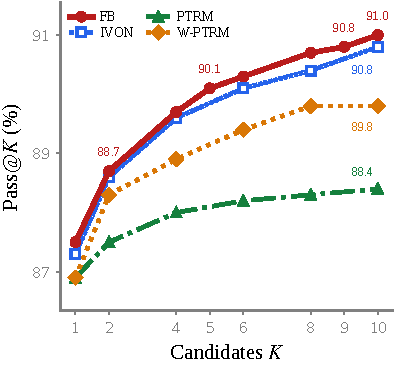
\includegraphics{figures/maze_hard_pass_at_k.pdf}
    \caption{Candidate coverage.}
    \label{fig:maze-hard-pass-at-k}
  \end{subfigure}\hfill
  \begin{subfigure}[t]{0.48\linewidth}
    \centering
    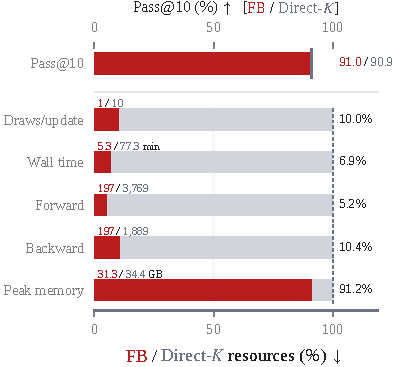
\includegraphics{figures/maze_hard_training_efficiency.pdf}
    \caption{Training resources.}
    \label{fig:maze-hard-training-efficiency}
  \end{subfigure}
  \caption{\textbf{FB improves inference and training efficiency on
  Maze-Hard.} (a) FB reaches each baseline's Pass@10 with fewer candidates
  using the same TRM backbone, 1,000 test problems, and reasoning depth 16.
  (b) At 188 updates, one-draw FB maintains comparable Pass@10 to
  Direct-$K{=}10$ while reducing training resources. Direct-$K$ uses seed 0;
  FB reports the mean over seeds 0--2.}
  \label{fig:maze-hard-efficiency}
\end{figure}

Using all saved FB prefixes to locate the first crossing, FB reaches PTRM's
Pass@10 of 88.4\% with two candidates, reducing solver executions by 80\%, and
reaches W-PTRM's 89.8\% with five candidates, reducing them by 50\%. FB also
reaches IVON's Pass@10 of 90.8\% with nine candidates, reducing solver
executions by 10\%; across the displayed budgets, FB exceeds IVON by
0.1--0.3 percentage points.

\subsection{Fidelity of one-draw finite-$K$ optimization}
\label{sec:objective-approximation}

We test whether one-draw FB follows the original finite-$K$ objective during
training.
\placeholder{Compare direct $K$-draw optimization, the naive one-sample
surrogate, and FB from matched initialization and training data. Add a
three-panel figure reporting (a) the true finite-$K$ objective estimated with
multiple posterior draws, (b) the saddle-objective gap, and (c) dual tracking
error over training.}

\subsection{Computational advantage of one-draw training}
\label{sec:computational-efficiency}

Direct finite-$K$ optimization requires $K$ solver executions per update,
whereas FB uses one.
At the matched endpoint of 188 updates,
\Cref{fig:maze-hard-training-efficiency} compares Direct-$K{=}10$ seed 0 with
the mean of FB seeds 0--2. FB attains 91.0\% Pass@10 versus 90.9\% for
Direct-$K$, while using 10.0\% as many posterior draws per update, 6.9\% of
the wall-clock time, 5.2\% of the forward passes, and 10.4\% of the backward
passes. Peak memory is reduced more modestly to 91.2\%. This endpoint
comparison supports comparable performance with substantially less training
compute; it does not establish a cost-to-target result.

\section{Limitations}
\label{sec:limitations}

Our analysis and experiments focus on a controlled setting for finite-$K$ posterior learning.
The binary all-fail probability is exact, as is the Fenchel representation of the differentiable finite-$K$ objective.
Practical training uses a differentiable failure score $f$ and a lagged per-problem failure estimate, so its agreement with binary coverage and the finite-$K$ gradient depends on the choice of $f$ and tracking accuracy, respectively.
We also assume fixed $K$ and $D$, independent posterior draws, and a retained selector, leaving adaptive budgets, correlated candidates, and joint selector training for future work.
Maintaining one failure estimate per training problem suits revisited finite datasets but may require amortization for very large or streaming data.
Finally, although the formulation supports any differentiably reparameterizable posterior, our experiments use IVON's diagonal Gaussian on two recursive reasoning backbones and a limited set of structured reasoning tasks.
Further evaluation is needed to establish whether the gains transfer to richer posterior families and larger language-based reasoning models.

\section{Conclusion}
\label{sec:conclusion}

We introduced finite-$K$ posterior learning, which trains a regularized posterior over solver parameters for the collective success of the candidate pool used at inference.
Starting from the exact probability that all $K$ posterior-sampled solvers fail, we define a differentiable objective aligned with candidate coverage under a fixed inference budget.
An exact Fenchel reformulation turns the posterior-dependent term into a one-draw expectation for a fixed problem-specific weight, and a closed-form Bregman update tracks that weight through running failure estimates.
The resulting procedure uses one solver execution per training update regardless of the candidate-pool size.
Across the tested reasoning tasks, our method improves candidate coverage and selected accuracy.
In a controlled Maze-Hard comparison, it achieves endpoint performance comparable to direct multi-draw training with substantially lower training cost.
These results support finite-$K$ posterior learning as a practical way to align posterior training with multi-sample inference without $K$-fold solver execution per update.


\bibliographystyle{unsrtnat}
\bibliography{main}

\clearpage
\appendix

\section{Finite-$K$ and dual-state derivations}
\label{app:proofs}

\subsection{Binary all-fail probability and direct Monte Carlo estimation}
\label{app:finite-k-details}

\paragraph{Probability space.}
Fix a problem $x$.
The problem is held fixed in the conditional probability below; randomness comes from drawing solver parameters from $q_\phi$.
For one draw $\theta\sim q_\phi$, the map $F(\theta,x)\in\{0,1\}$ is deterministic once $\theta$ and $x$ are fixed, but it is a random variable before $\theta$ is drawn.
Every binary random variable is Bernoulli, so $F(\theta,x)$ has failure probability
\begin{equation}
  \Pr_{\theta\sim q_\phi}\!\left(F(\theta,x)=1\right)
  =
  \mathbb E_{\theta\sim q_\phi}[F(\theta,x)].
  \label{eq:app-one-draw-failure}
\end{equation}
The equality follows from the indicator identity $\mathbb E[\mathbf 1\{A\}]=\Pr(A)$.
It does not require $F(\theta,x)$ to output a calibrated probability: $F$ only records whether the sampled solver fails.

\paragraph{The all-fail event.}
At inference, draw $\theta_{1:K}\overset{\mathrm{iid}}{\sim}q_\phi$.
For each $k$, define the failure event $A_k(x)=\{F(\theta_k,x)=1\}$.
The event that all $K$ sampled solvers fail is the intersection $A_{1:K}(x)=\bigcap_{k=1}^K A_k(x)$.
Because each $F(\theta_k,x)$ is binary, the indicator of this intersection is
\begin{equation}
  \mathbf 1\{A_{1:K}(x)\}
  =
  \prod_{k=1}^K \mathbf 1\{A_k(x)\}
  =
  \prod_{k=1}^K F(\theta_k,x).
  \label{eq:app-all-fail-indicator}
\end{equation}
The product is one only when every factor is one, and it is zero as soon as one sampled solver succeeds.
Taking its expectation therefore gives the all-fail probability:
\begin{align}
  &\Pr_{\theta_{1:K}\overset{\mathrm{iid}}{\sim}q_\phi}
  (\text{all $K$ solvers fail}\mid x)
  \notag\\
  &\quad=
  \mathbb E_{\theta_{1:K}\overset{\mathrm{iid}}{\sim}q_\phi}
  \left[\mathbf 1\{A_{1:K}(x)\}\right]
  \notag\\
  &\quad=
  \mathbb E_{\theta_{1:K}\overset{\mathrm{iid}}{\sim}q_\phi}
  \left[\prod_{k=1}^K F(\theta_k,x)\right].
  \label{eq:app-all-fail-expectation}
\end{align}
This identity explains why the product appears inside an expectation.
It holds for any joint distribution of $\theta_{1:K}$; independence is not needed until the next step.

\paragraph{Factorization under independent sampling.}
The prescribed inference protocol samples each $\theta_k$ independently from the same posterior.
Its joint distribution is therefore the product measure $q_\phi^{\otimes K}$.
Independence factors the expectation in \cref{eq:app-all-fail-expectation}:
\begin{align}
  &\mathbb E_{\theta_{1:K}\overset{\mathrm{iid}}{\sim}q_\phi}
  \left[\prod_{k=1}^K F(\theta_k,x)\right]
  \notag\\
  &\quad=
  \prod_{k=1}^K
  \mathbb E_{\theta_k\sim q_\phi}[F(\theta_k,x)]
  \notag\\
  &\quad=
  \left(
    \mathbb E_{\theta\sim q_\phi}[F(\theta,x)]
  \right)^K.
  \label{eq:app-binary-finite-k}
\end{align}
The first equality uses independence, while the second uses the fact that all draws have the same distribution.
Equivalently, the same factorization can be read directly as a product of $K$ identical one-draw failure probabilities from \cref{eq:app-one-draw-failure}.
Combining \cref{eq:app-all-fail-expectation,eq:app-binary-finite-k} gives the main-text identity in \cref{eq:binary-all-fail}.

\paragraph{Candidate coverage and Pass@$K$.}
The event that the pool contains at least one successful solver is the complement of the all-fail event.
Under the same sampling protocol,
\begin{equation}
  \Pr(\text{at least one of the $K$ solvers succeeds}\mid x)
  =
  1-
  \left(
    \mathbb E_{\theta\sim q_\phi}[F(\theta,x)]
  \right)^K.
  \label{eq:app-pass-k}
\end{equation}
This probability is the candidate-coverage or Pass@$K$ target used in the paper.
It measures whether the pool contains a correct candidate; it does not model whether the retained selector identifies that candidate.
The outer expectation over $x$ in \cref{eq:exact-finite-k-objective} averages this conditional all-fail probability over the problem distribution.

\paragraph{Direct Monte Carlo estimator for the binary target.}
One independently sampled pool $\theta_{1:K}$ yields
\begin{equation}
  \widehat R_K^{F}(x;\theta_{1:K})
  =
  \prod_{k=1}^K F(\theta_k,x).
  \label{eq:app-hard-direct-estimator}
\end{equation}
By \cref{eq:app-all-fail-expectation}, this estimator is unbiased for the exact all-fail probability.
It is itself binary: it returns one when the sampled pool contains no successful solver and zero otherwise.
Computing it requires executing all $K$ sampled solvers.

\paragraph{Differentiable replacement.}
The hard indicator $F$ does not provide the pathwise gradient used to train the posterior.
We replace it with the differentiable failure score $f(\theta,x)\in[0,1]$ and define $\bar f_\phi(x)=\mathbb E_{\theta\sim q_\phi}[f(\theta,x)]$.
For $K$ independent posterior draws, define the direct estimator
\begin{equation}
  \widehat R_K^{f}(x;\theta_{1:K})
  =
  \prod_{k=1}^K f(\theta_k,x).
  \label{eq:app-soft-direct-estimator}
\end{equation}
Independence gives
\begin{align}
  \mathbb E_{\theta_{1:K}\overset{\mathrm{iid}}{\sim}q_\phi}
  [\widehat R_K^{f}(x;\theta_{1:K})]
  & =
  \prod_{k=1}^K
  \mathbb E_{\theta_k\sim q_\phi}[f(\theta_k,x)]
  \notag\\
  & =
  \bar f_\phi(x)^K.
  \label{eq:app-soft-finite-k}
\end{align}
Thus, the $K$-draw product is an unbiased estimator of the differentiable finite-$K$ data term.
Unlike \cref{eq:app-hard-direct-estimator}, the soft product in \cref{eq:app-soft-direct-estimator} is not an event indicator.
Consequently, $\bar f_\phi(x)^K$ is a smooth training target rather than a literal all-fail probability unless $f=F$ or $f$ has an additional probabilistic interpretation.

\paragraph{Why one draw cannot be reused directly.}
Suppose that one posterior draw is used in all $K$ factors.
The resulting estimator is $f(\theta,x)^K$, whose expectation is
\begin{equation}
  \mathbb E_{\theta\sim q_\phi}[f(\theta,x)^K],
  \label{eq:app-reused-draw}
\end{equation}
not $\bar f_\phi(x)^K$.
For $K>1$, the map $u\mapsto u^K$ is convex on $[0,1]$, so Jensen's inequality gives
\begin{equation}
  \mathbb E_{\theta\sim q_\phi}[f(\theta,x)^K]
  \geq
  \left(
    \mathbb E_{\theta\sim q_\phi}[f(\theta,x)]
  \right)^K.
  \label{eq:app-reused-draw-jensen}
\end{equation}
For $K>1$, equality holds when $f(\theta,x)$ is constant almost surely under $q_\phi$; it need not hold during posterior learning.
In the binary case, $F(\theta,x)^K=F(\theta,x)$, so reusing one draw estimates the one-draw failure probability rather than the $K$-draw all-fail probability.
This distinction motivates the Fenchel representation in \cref{app:fenchel-proof}: it preserves the finite-$K$ target while making the posterior-dependent update estimable with one fresh draw for a fixed dual state.

\paragraph{Scope of the derivation.}
The $K$-th power in \cref{eq:binary-all-fail,eq:app-binary-finite-k} relies on independent posterior draws.
If the candidate solvers are sampled jointly with correlation, \cref{eq:app-all-fail-expectation} remains valid, but the expectation does not generally factor into a $K$-th power.
Our notation also treats solver execution as deterministic conditional on $(\theta,x)$.
If the solver uses additional randomness $\xi$, one may instead write $F(\theta,\xi,x)$ and draw the pairs $(\theta_k,\xi_k)$ independently; the same derivation then applies to the augmented sampling distribution.

\subsection{Derivation of the Fenchel representation}
\label{app:fenchel-proof}

For $K\geq2$, consider $h_r(\lambda)=\lambda r-\psi_K(\lambda)$ on $[0,K]$.
Its derivative on $(0,K)$ is
\begin{equation}
  h_r'(\lambda)
  =
  r-\left(\frac{\lambda}{K}\right)^{1/(K-1)}.
  \label{eq:app-fenchel-derivative}
\end{equation}
The unique stationary point is $\lambda^\star(r)=Kr^{K-1}$, which lies in $[0,K]$ for $r\in[0,1]$.
Substitution gives
\begin{equation}
  h_r(\lambda^\star(r))
  =
  Kr^{K-1}r-(K-1)r^K
  =
  r^K.
  \label{eq:app-fenchel-substitution}
\end{equation}
Because $\psi_K$ is strictly convex, $h_r$ is strictly concave and this stationary point is the unique maximizer for $r\in(0,1)$.
The boundary cases give $\lambda^\star(0)=0$ and $\lambda^\star(1)=K$.
The case $K=1$ needs no Fenchel step because the objective is linear in $r$.

\subsection{Fixed-dual one-draw gradient}
\label{app:fixed-dual-gradient}

Assume that $q_\phi$ admits a differentiable reparameterization $\theta=T_\phi(\epsilon)$ whose base distribution does not depend on $\phi$.
Also assume that an integrable dominating function permits differentiation under the expectation.
For a fixed detached dual state $\lambda_x$,
\begin{align}
  \nabla_\phi\mathbb E_{q_\phi}[\lambda_x f(\theta,x)]
  &=
  \nabla_\phi\mathbb E_\epsilon[\lambda_x f(T_\phi(\epsilon),x)]
  \notag\\
  &=
  \mathbb E_\epsilon[\nabla_\phi\{\lambda_x f(T_\phi(\epsilon),x)\}].
  \label{eq:app-fixed-dual-gradient}
\end{align}
One draw of $\epsilon$, or equivalently one $\theta\sim q_\phi$, therefore gives an unbiased stochastic gradient of the fixed-dual data term.
Moreover,
\begin{equation}
  \nabla_\phi\bar f_\phi(x)^K
  =
  K\bar f_\phi(x)^{K-1}\nabla_\phi\bar f_\phi(x)
  =
  \lambda^\star(\bar f_\phi(x))\nabla_\phi\bar f_\phi(x).
  \label{eq:app-finite-k-gradient}
\end{equation}
The fixed-dual gradient coincides with the finite-$K$ data gradient when $\lambda_x=\lambda^\star(\bar f_\phi(x))$.
For a lagged dual state, unbiasedness holds conditionally for the fixed-dual objective.

\subsection{Dual coordinate and Bregman update}
\label{app:bregman-proof}

\begin{lemma}[Dual coordinate]
\label{lem:dual-coordinate}
For integer $K\geq2$ and $\lambda\in[0,K]$, the derivative $\psi_K'(\lambda)=(\lambda/K)^{1/(K-1)}$ is a strictly increasing bijection from $[0,K]$ to $[0,1]$.
Its inverse is $(\psi_K')^{-1}(u)=Ku^{K-1}$ for $u\in[0,1]$, and $\psi_K'(\lambda^\star(r))=r$.
\end{lemma}

\begin{proof}
Direct differentiation gives the stated derivative, including its continuous extension at zero.
The derivative increases from zero to one on $[0,K]$.
Solving $u=(\lambda/K)^{1/(K-1)}$ gives the inverse, and substituting $\lambda^\star(r)=Kr^{K-1}$ gives the final identity.
\end{proof}

\begin{proposition}[Bregman-proximal dual update]
\label{prop:bregman-update}
Let $K\geq2$, $\eta>0$, $\lambda_{x,t}\in[0,K]$, and $f_t\in[0,1]$.
If $\widehat f_{x,t-1}=\psi_K'(\lambda_{x,t})$ and $\beta=1/(1+\eta)$, then the unique maximizer in \cref{eq:dual-prox} is given by \cref{eq:dual-ema}.
\end{proposition}

\begin{proof}
Expanding the Bregman divergence in \cref{eq:dual-prox} and dropping terms independent of $\lambda$ gives
\begin{equation}
  Q_t(\lambda)
  =
  \left(f_t+\frac{\widehat f_{x,t-1}}{\eta}\right)\lambda
  -
  \left(1+\frac{1}{\eta}\right)\psi_K(\lambda)
  +\mathrm{const}.
  \label{eq:app-bregman-expanded}
\end{equation}
Strict convexity of $\psi_K$ makes $Q_t$ strictly concave.
The first-order condition gives
\begin{equation}
  \psi_K'(\lambda_{x,t+1})
  =
  \frac{\widehat f_{x,t-1}+\eta f_t}{1+\eta}
  =
  \beta\widehat f_{x,t-1}+(1-\beta)f_t.
  \label{eq:app-bregman-coordinate}
\end{equation}
The right-hand side lies in $[0,1]$, so \cref{lem:dual-coordinate} covers the interior and both boundary cases.
Applying $(\psi_K')^{-1}$ yields $\lambda_{x,t+1}=K\widehat f_{x,t}^{K-1}$.
\end{proof}

\subsection{Indexing and the lagged dual state}
\label{app:dual-indexing}

The implementation follows the order
\begin{equation}
  \widehat f_{x,t-1}
  \longrightarrow
  \lambda_{x,t}=K\widehat f_{x,t-1}^{K-1}
  \longrightarrow
  \theta_t\sim q_{\phi_t}
  \longrightarrow
  f_{x,t}
  \longrightarrow
  \widehat f_{x,t}.
  \label{eq:app-lagged-indexing}
\end{equation}
Let $\mathcal H_{t-1}$ denote the training history before drawing $\theta_t$.
The state $\lambda_{x,t}$ is measurable with respect to $\mathcal H_{t-1}$ and is fixed before the current posterior sample.
The one-draw gradient result therefore applies conditionally on this history.
Detaching a dual state formed from the current sample blocks its autograd path but does not make it statistically independent of that sample.
Using the lagged state avoids this dependence.

\subsection{Stationary stochastic tracking}
\label{app:stationary-tracking}

\begin{proposition}[Stationary stochastic tracking]
\label{prop:stationary-tracking}
Fix $K\geq2$ and $\beta\in(0,1)$.
Let $f_t\in[0,1]$ satisfy $\mathbb E[f_t\mid\mathcal H_{t-1}]=r$ and $\mathbb E[(f_t-r)^2\mid\mathcal H_{t-1}]\leq\sigma^2$ for fixed $r\in[0,1]$.
For $\widehat f_t=\beta\widehat f_{t-1}+(1-\beta)f_t$, $\lambda_{t+1}=K\widehat f_t^{K-1}$, and $\lambda^\star=Kr^{K-1}$,
\begin{align}
  \mathbb E[\widehat f_t]-r
  &=\beta^t(\widehat f_0-r),
  \label{eq:stationary-bias}\\
  \mathbb E[(\widehat f_t-r)^2]
  &\leq
  \beta^{2t}(\widehat f_0-r)^2
  +
  \sigma^2\frac{1-\beta}{1+\beta}(1-\beta^{2t}),
  \label{eq:stationary-mse}\\
  \mathbb E[(\lambda_{t+1}-\lambda^\star)^2]
  &\leq
  K^2(K-1)^2\mathbb E[(\widehat f_t-r)^2].
  \label{eq:stationary-dual}
\end{align}
The Fenchel inner-max gap $\Delta_t=r^K-[\lambda_{t+1}r-\psi_K(\lambda_{t+1})]$ satisfies
\begin{equation}
  0\leq\mathbb E[\Delta_t]
  \leq
  \frac{K(K-1)}{2}\mathbb E[(\widehat f_t-r)^2].
  \label{eq:stationary-gap}
\end{equation}
\end{proposition}

\begin{proof}
Set $e_t=\widehat f_t-r$ and $\xi_t=f_t-r$.
Then $e_t=\beta e_{t-1}+(1-\beta)\xi_t$ and $\mathbb E[\xi_t\mid\mathcal H_{t-1}]=0$.
Taking expectations gives \cref{eq:stationary-bias}.
Squaring, conditioning, and unrolling the resulting recursion gives \cref{eq:stationary-mse}.
For $g(u)=Ku^{K-1}$ on $[0,1]$, the bound $|g'(u)|\leq K(K-1)$ and the mean-value theorem give \cref{eq:stationary-dual}.
Finally, $\psi_K'(\lambda^\star)=r$ implies $\Delta_t=D_{\psi_K}(\lambda_{t+1},\lambda^\star)$.
Writing $u=\widehat f_t$ and integrating the derivative of $r^K-Kru^{K-1}+(K-1)u^K$ between $r$ and $u$ gives \cref{eq:stationary-gap}.
\end{proof}

\subsection{Non-stationary stochastic tracking}
\label{app:nonstationary-tracking}

\begin{proposition}[Non-stationary stochastic tracking]
\label{prop:nonstationary-tracking}
Fix $K\geq2$ and $\beta\in(0,1)$.
Let $r_t=\mathbb E[f_t\mid\mathcal H_{t-1}]$, $\xi_t=f_t-r_t$, and $\mathbb E[\xi_t^2\mid\mathcal H_{t-1}]\leq\sigma_t^2$.
Define $e_t=\widehat f_{t-1}-r_t$, $\lambda_t=K\widehat f_{t-1}^{K-1}$, and $\lambda_t^\star=Kr_t^{K-1}$.
Then
\begin{equation}
  e_t
  =
  \beta^{t-1}e_1
  +(1-\beta)\sum_{j=1}^{t-1}\beta^{t-1-j}\xi_j
  -\sum_{j=1}^{t-1}\beta^{t-1-j}(r_{j+1}-r_j).
  \label{eq:nonstationary-recursion}
\end{equation}
Consequently,
\begin{align}
  \|e_t\|_2
  &\leq
  \beta^{t-1}\|e_1\|_2
  +
  \sum_{j=1}^{t-1}\beta^{t-1-j}\|r_{j+1}-r_j\|_2
  \notag\\
  &\quad+
  (1-\beta)
  \left(\sum_{j=1}^{t-1}\beta^{2(t-1-j)}\sigma_j^2\right)^{1/2}.
  \label{eq:nonstationary-bound}
\end{align}
If $\|r_{t+1}-r_t\|_2\leq\delta$ and $\sigma_t\leq\sigma$, then
\begin{equation}
  \limsup_{t\to\infty}\|e_t\|_2
  \leq
  \frac{\delta}{1-\beta}
  +
  \sigma\sqrt{\frac{1-\beta}{1+\beta}}.
  \label{eq:nonstationary-limit}
\end{equation}
With $\rho_t=\max\{\widehat f_{t-1},r_t\}$, the dual error and instantaneous Fenchel gap $\Gamma_t=r_t^K-[\lambda_t r_t-\psi_K(\lambda_t)]$ satisfy
\begin{align}
  |\lambda_t-\lambda_t^\star|
  &\leq K(K-1)\rho_t^{K-2}|e_t|,
  \label{eq:nonstationary-dual}\\
  0\leq\Gamma_t
  &\leq\frac{K(K-1)}{2}\rho_t^{K-2}e_t^2.
  \label{eq:nonstationary-gap}
\end{align}
\end{proposition}

\begin{proof}
The EMA recursion gives $e_{t+1}=\beta e_t+(1-\beta)\xi_t-(r_{t+1}-r_t)$.
Unrolling it yields \cref{eq:nonstationary-recursion}.
The martingale-difference property removes cross terms in the squared norm of the noise sum.
The triangle inequality in $L_2$ then gives \cref{eq:nonstationary-bound}.
Bounding the drift and noise terms by geometric series gives \cref{eq:nonstationary-limit}.
Factoring the difference between $\widehat f_{t-1}^{K-1}$ and $r_t^{K-1}$ gives \cref{eq:nonstationary-dual}.
The identity $\Gamma_t=D_{\psi_K}(\lambda_t,\lambda_t^\star)$ and the same integral argument as in \cref{prop:stationary-tracking} give \cref{eq:nonstationary-gap}.
\end{proof}

The bounds separate sampling noise from drift in the posterior failure rate.
Increasing $\beta$ reduces the noise term but increases the lag term $\delta/(1-\beta)$.
These results guarantee tracking of the dual state, not convergence of the full neural-network optimization.

\section{Experimental details}
\label{app:experimental-details}

\subsection{Datasets and evaluation protocols}

\placeholder{Report dataset splits, preprocessing, reasoning depth, selectors,
the distinction between $K_{\mathrm{train}}$ and $K_{\mathrm{eval}}$, evaluation
seeds, and confidence-interval construction for Sudoku-Extreme, Maze-Hard,
and ARC-AGI-2.}

\paragraph{Maze-Hard candidate-coverage protocol.}
We evaluate FB, ordinary IVON, PTRM, and W-PTRM on the same 1,000-problem test
split with the TRM backbone, reasoning depth 16, and candidate budgets up to
ten. All four methods use ordered prefixes from saved
$K_{\mathrm{eval}}=10$ banks under seed-0 reset sampling. For IVON, we
evaluate the EMA model state stored in the seed-0 checkpoint.

\subsection{Baseline details}

\paragraph{Deterministic reasoning models.}
\textbf{HRM} couples recurrent modules that operate at different time
scales~\citep{wang2025hierarchical}. \textbf{TRM} replaces the hierarchy with
one small recursive network~\citep{jolicoeurmartineau2025trm}.
\textbf{FPRM} uses fixed-point convergence to halt a looped
Transformer~\citep{movahedi2026fixedpoint}.

\paragraph{Sampling-based reasoning methods.}
\textbf{GRAM} models reasoning as stochastic latent trajectories and samples
several trajectories in parallel~\citep{baek2026generative}. \textbf{PTRM}
keeps the model parameters fixed, injects Gaussian noise into the latent state
at each deep-recursion step, and selects among the resulting
trajectories~\citep{sghaier2026probabilistic}. \textbf{W-PTRM} and
\textbf{W-FPRM} are non-learned baselines that sample each candidate's
parameters from a fixed Gaussian centered at the released TRM or FPRM
checkpoint. They add no latent noise.

\paragraph{Posterior optimization methods.}
\textbf{IVON} (Improved Variational Online Newton) maintains a sampleable
diagonal Gaussian through an online variational update and optimizes the
single-draw posterior objective~\citep{shen2024variational}. \textbf{FB
(Ours)} uses the same IVON posterior parameterization and initialization, but
optimizes the finite-$K$ objective with Fenchel--Bregman updates. For learned
posterior methods, we initialize the posterior mean from a released task
checkpoint and fine-tune its mean and diagonal precision on the task training
split. Fine-tuning adapts the solver distribution to the chosen objective,
while W-PTRM and W-FPRM isolate sampling without this adaptation.

\subsection{Training and compute accounting}

\placeholder{Report optimization hyperparameters, posterior and dual-state
initialization, training-update budgets, hardware, batch sizes, mixed-precision
settings, solver-call accounting, wall-clock measurement, and peak-memory
measurement.}

\paragraph{Ordinary-IVON baseline.}
Ordinary IVON uses the shared released-checkpoint initialization, task data,
update budget, and fixed $K=10$ test protocol described above.

\section{Additional posterior analyses}
\label{app:posterior-analysis}

\subsection{Posterior learning across recursive backbones}
\label{sec:cross-backbone}

\Cref{tab:maze-cross-backbone} compares posterior methods with TRM and FPRM backbones on the complete Maze-Hard test set.
Every stochastic method uses ten candidates ($K=10$) and its native selector.

\begin{table}[t]
  \caption{\textbf{FB obtains the highest selected accuracy and Pass@10
  with both backbones on Maze-Hard.} Results are percentages on the complete
  1,000-puzzle test set. Bold and underlined values mark the best and
  second-best results within each backbone.}
  \label{tab:maze-cross-backbone}
  \centering
  \small
  \setlength{\tabcolsep}{22pt}
  \begin{adjustbox}{max width=1.0\linewidth}
  \begin{tabular}{lcc}
    \toprule
    Method & Acc. $\uparrow$ & Pass@10 $\uparrow$ \\
    \midrule
    \multicolumn{3}{l}{\textit{TRM backbone}} \\
    Deterministic            & 87.00 & 87.00 \\
    PTRM                     & \underline{87.70} & 88.40 \\
    W-PTRM                   & 87.50 & \underline{89.80} \\
    \rowcolor{gaerowhighlight}
    \textbf{FB (Ours)}       & \textbf{88.00} & \textbf{91.00} \\
    \addlinespace
    \multicolumn{3}{l}{\textit{FPRM backbone}} \\
    Deterministic            & \underline{86.90} & -- \\
    W-FPRM                   & \underline{86.90} & 88.70 \\
    IVON                     & 84.40 & \underline{94.00} \\
    \rowcolor{gaerowhighlight}
    \textbf{FB (Ours)}       & \textbf{87.70} & \textbf{94.80} \\
    \bottomrule
  \end{tabular}
  \end{adjustbox}
\end{table}

FB improves both metrics under the two tested backbones.
With TRM, it raises selected accuracy by 0.30 percentage points over PTRM and Pass@10 by 1.20 points over W-PTRM.
With FPRM, FB improves selected accuracy from 84.40\% to 87.70\% and Pass@10 from 94.00\% to 94.80\% over IVON.
The paired 95\% bootstrap intervals are [1.60, 5.10] for selected accuracy and [0.00, 1.60] for Pass@10.
The two FPRM posterior rows use the same initialization, training data, update budget, and evaluation noise.

\subsection{Posterior construction under a fixed backbone}
\label{sec:posterior-construction}

\Cref{tab:posterior-construction} fixes the FPRM backbone and Maze-Hard protocol while varying how each method constructs its parameter distribution.
Diagonal Laplace fits a local Gaussian from curvature at a point estimate~\citep{daxberger2021laplace}, while SWAG estimates a Gaussian from an SGD trajectory~\citep{maddox2019swag}.

\begin{table}[h]
  \caption{\textbf{The comparison fixes FPRM and Maze-Hard while varying
  the posterior construction.}}
  \label{tab:posterior-construction}
  \centering
  \small
  % \begin{adjustbox}{width=1.0\linewidth}
  \begin{tabular}{lcc}
    \toprule
    Method &  Acc. $\uparrow$ & Pass@10 $\uparrow$ \\
    \midrule
    FPRM                    & \underline{86.90} & -- \\
    W-FPRM                  & \underline{86.90} & 88.70 \\
    Diagonal Laplace        & \pendingcell{Diagonal Laplace Acc.} & \pendingcell{Diagonal Laplace Pass@10} \\
    SWAG                    & \pendingcell{SWAG Acc.} & \pendingcell{SWAG Pass@10} \\
    IVON                    & 84.40 & \underline{94.00} \\
    \rowcolor{gaerowhighlight}
    \textbf{FB (Ours)}      & \textbf{87.70} & \textbf{94.80}\\
    \bottomrule
  \end{tabular}
  % \end{adjustbox}
\end{table}

Among posterior results, FB improves selected accuracy by 3.30 percentage points and Pass@10 by 0.80 points over IVON.
\resultpending{Compare FB with Diagonal Laplace and SWAG after their matched Maze-Hard results and fit times are available.}

\paragraph{Candidate diversity.}
\placeholder{Report the unique-solution ratio and candidate disagreement for
each posterior method. Pair each diversity statistic with Pass@$K$ so that
output variation is not interpreted as useful coverage by itself.}


\section{Additional objective and resource analyses}
\label{app:additional-objective-resource}

\subsection{Extended objective and tracking diagnostics}

\placeholder{Report the naive one-sample surrogate, detailed saddle-objective
gap, per-problem and aggregate dual tracking errors, and sensitivity of the
tracking gap over training.}

\subsection{Extended inference-budget results}

\placeholder{Report all saved prefixes for $K=1,\ldots,10$, per-seed results,
confidence intervals, and additional sampling baselines that do not fit in
the main figure.}


\section{Ablation studies}
\label{app:ablations}

\paragraph{EMA coefficient.}
\placeholder{Evaluate $\beta\in\{0,0.9,0.99,0.999\}$ using dual tracking
error, the final finite-$K$ objective, optimization stability, and Pass@$K$.
Relate smaller $\beta$ to responsive but noisy estimates and larger $\beta$
to smoother but slower tracking.}

\paragraph{Other optimization choices.}
\placeholder{Report ablations for the KL coefficient $\tau_{\mathrm{KL}}$,
dual-state initialization, and $K_{\mathrm{train}}$. Include the final
finite-$K$ objective, tracking error, Pass@$K$, and selected accuracy where
applicable.}



\end{document}
